{\chapter{Das Online-Matching-Problem}

\section{Deterministische Algorithmen}

\textbf{Theorem 7.1.} Jeder Greedy-Algorithmus, der nach dem oben beschriebenen Prinzip arbeitet, ist strikt 2-kompetitiv für das Online-Matching-Problem.

\textit{Beweis:} Jeder Greedy-Algorithmus berechnet einen nicht erweiterbares Matching, da er ansonsten die Kante, als sie durch die Eingabe möglich geworderden ist, als in das Matching mit einbezogen hätte (dies entsspricht der Eigenschaft von diesem Greedy-Algorithmus).

Zum Beweis fehlen noch folgende Aussagen: ($M$ ist bel. nicht erweiterbares Matching; $M^{*}$ maximales Matching)
\begin{itemize}
\item $|M^{*}| \le 2|M|$ (jede Kante aus $M$ kann max 2 aus $M^{*}$ verdrängen)
\item $|V(M)| = 2|M|$
\item $|V(M^{*}| = 2|M^{*}|)$
\item $|V(M)| \ge |M^{*}|$
\end{itemize}
Daraus folgt: $$|M| = \frac{|V(M)|}{2} \ge \frac{|M^{*}}{2}$$

\textbf{Theorem 7.2.} Es gibt keinen deterministischen Online-Algorithmus für das Online-Matching-Problem, der einen besseren kompetitiven Faktor als 2 erreicht.

\textit{Beweis:} Gegenbeispiel:\\
Wir haben $v_{1}, v_{2}$ gegeben. Wenn Knoten $u_{1}$ aufgedeckt wird und diese Kanten jeweils zu $v_{1}$ und $v_{2}$ wird der Algorithmus eine der beiden Kanten zum Matching hinzufügen. Dieses Verhalten kann leicht ausgetrickst werden, indem $u_{2}$ nur zu dem Knoten eine Kante hat, der bereits dem Matching angehört. Das maximale Matching wäre in dem Fall 2, der deterministische Algorithmus bekommt aber nur 1.

Um den konstanten Faktor $\tau$ zu entfernen, wiederholen wir dies beliebig oft, sodass $\tau$ keine Rolle mehr spielt.

\section{Randomisierte Algorithmen}

\textit{RANDOM (randomisierter Greedy-Algorithmus):} RANDOM wählt beim Aufdecken eines Knotens u $\in$ U uniform zufällig einen Knoten v $\in$ V aus der Menge aller noch freien Nacharn von u aus und weist dann u und v einander zu.

\textbf{Theorem 7.3.} Es gibt keine Konstante $r < 2$, für die der Algorithmus RANDOM r-kompetitiv ist.

\textit{Beweis:} 

\begin{figure}[h]
  \centering
  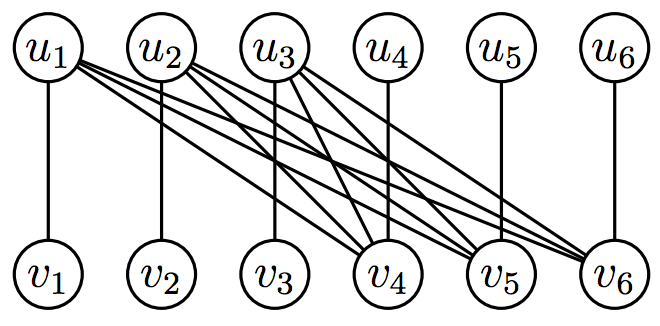
\includegraphics[width=0.4\textwidth]{7_3}
  \caption{Zuordnung der Knoten}
\end{figure}
$$E[|M|] = n + E[x] = n + \sum_{i=1}^{n} p_{i} $$
$$E[X] = \sum_{i=1}^{n} \le \sum_{i=1}^{n} \frac{1}{n - i + 2} = ... \le ln(n) + 1$$

\textit{RANKING (leichte Abwandlung von RANDOM):}

\textbf{Theorem 7.4.} Der Algorithmus RANKING ist auf Graphen, in denen das maximale Matching die Größe n besitzt, strikt $\tfrac{1}{1-(1-\tfrac{1}{n+1})^{n}}$-kompetitiv.

\textit{Beweis:} Nicht relevant, haben wir in der Vorlesung übersprungen (glaub ich)

\textbf{Lemma 7.5.} Es sei $\sigma$ eine beliebige Permutation der Menge V, x $\in V \cup V$ ein beliebiger Knoten und H der Graph, der aus G entsteht, indem der Knoten x und alle zu ihm inzidenten Kanten entfernt werden. Dann sind die Matchings M = RANKING(G, $\sigma$) und M' = RANKING(H, $\sigma_{x}$) entweder identisch oder sie unterscheiden sich um einen M-alternierenden Pfad P, der mindestens so viele Kanten aus M wie E \ M enthält. Dabei bezeichne $\sigma_{x}$ die Permutation, die $\sigma$ auf V \textbackslash \{x\} durch Löschen von x induziert (für x $\in$ U gilt $\sigma = \sigma_{x}$), und wir gehen davon aus, dass die Knoten aus U\textbackslash \{x\} in dem Graph H in derselben Reihenfolge ankommen wie in G.

\textit{Beweis:}
\begin{figure}[h]
  \centering
  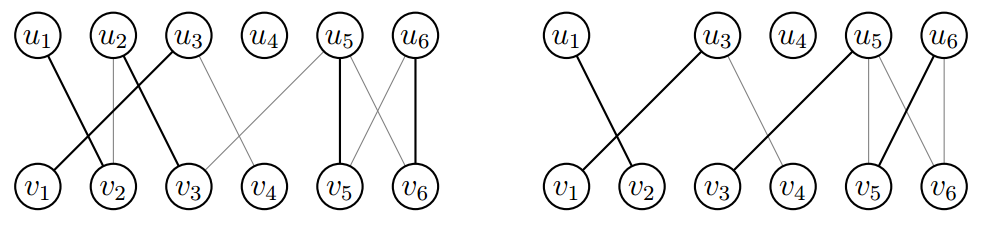
\includegraphics[width=0.8\textwidth]{7_5}
  \caption{Zuordnung der Knoten}
\end{figure}

\textbf{Lemma 7.6.} Es sei u $\in$ U beliebig und es sei v = $m^{*}(u)$. Falls der Knoten v in dem Matching M nicht zugewiesen ist, so ist u in M einen knoten zugewiesen, dessen Rang kleiner ist als der von v.

\textit{Beweis:} !!!!!TODO!!!!!

\textbf{Lemma 7.7.} Für t $\in$ \{1, ..., n\} gilt: $1 - p_{t} \le \tfrac{1}{n} \sum_{s=1}^{t} p_{s}$.

\textit{Beweis:} !!!!!TODO!!!!!

